\documentclass[tikz,border=7pt]{standalone}
% Shared visual language for the book's standalone vector figures.
% Keep this file compatible with the TeX Live version used by LyX.
\usepackage{amsmath,amssymb}
\usepackage{array,booktabs}
\usepackage{pgfplots}
\usepackage{pgfplotstable}
\usetikzlibrary{arrows.meta,calc,positioning}
\pgfplotsset{compat=1.17}

\definecolor{BookBlue}{HTML}{0072B2}
\definecolor{BookOrange}{HTML}{D55E00}
\definecolor{BookGreen}{HTML}{009E73}
\definecolor{BookGray}{HTML}{666666}
\definecolor{BookLightGray}{HTML}{D9D9D9}

\pgfplotsset{
  book axis/.style={
    axis line style={black!75,line width=0.55pt},
    tick style={black!75,line width=0.45pt},
    tick label style={font=\small},
    label style={font=\small},
    legend style={
      font=\small,
      draw=none,
      fill=none,
      cells={anchor=west},
    },
    grid style={BookLightGray,line width=0.35pt},
    major grid style={BookLightGray,line width=0.35pt},
  },
}

\begin{document}
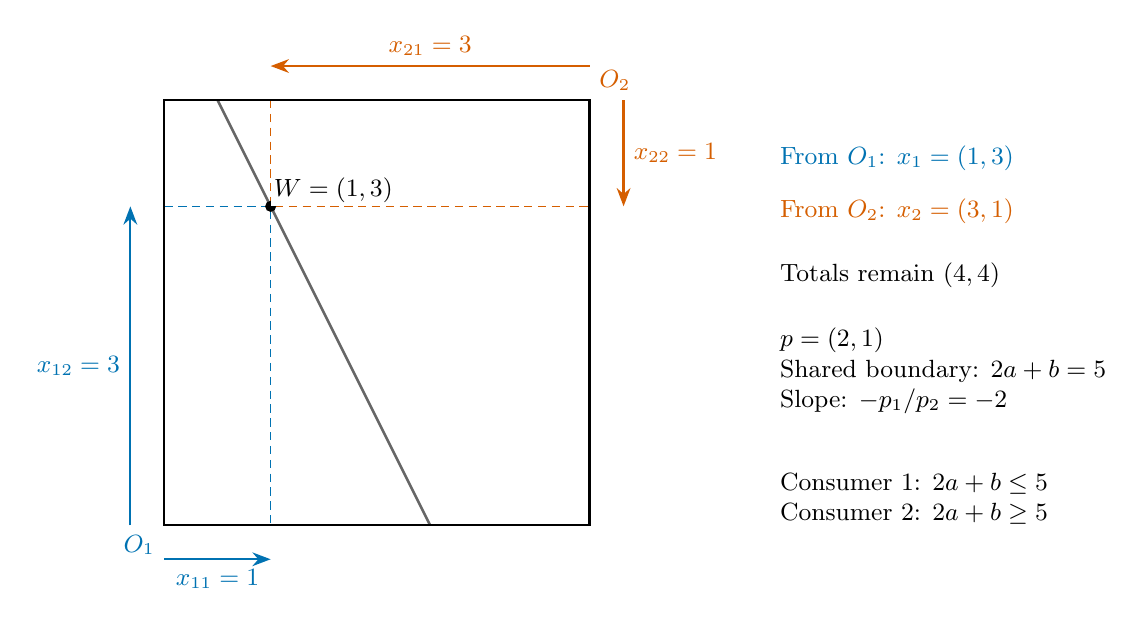
\begin{tikzpicture}[x=1.35cm,y=1.35cm,>=Stealth,font=\small]
  % One physical allocation is read from two opposite origins.
  % The price example explains budgets; it is not an equilibrium claim.
  \draw[BookGray,line width=.9pt] (.5,4)--(2.5,0);
  \draw[BookBlue,densely dashed] (0,3)--(1,3)--(1,0);
  \draw[BookOrange,densely dashed] (1,4)--(1,3)--(4,3);
  \draw[thick] (0,0) rectangle (4,4);
  \node[below left,BookBlue] at (0,0) {$O_1$};
  \node[above right,BookOrange] at (4,4) {$O_2$};
  \draw[->,BookBlue,thick] (0,-.32)--(1,-.32)
    node[midway,below] {$x_{11}=1$};
  \draw[->,BookBlue,thick] (-.32,0)--(-.32,3)
    node[midway,left] {$x_{12}=3$};
  \draw[->,BookOrange,thick] (4,4.32)--(1,4.32)
    node[midway,above] {$x_{21}=3$};
  \draw[->,BookOrange,thick] (4.32,4)--(4.32,3)
    node[midway,right] {$x_{22}=1$};
  \fill (1,3) circle(2pt)
    node[above right,fill=white,inner sep=1pt] {$W=(1,3)$};
  \node[anchor=west,BookBlue] at (5.7,3.45) {From $O_1$: $x_1=(1,3)$};
  \node[anchor=west,BookOrange] at (5.7,2.95) {From $O_2$: $x_2=(3,1)$};
  \node[anchor=west] at (5.7,2.35) {Totals remain $(4,4)$};
  \node[anchor=west,align=left] at (5.7,1.45)
    {$p=(2,1)$\\Shared boundary: $2a+b=5$\\Slope: $-p_1/p_2=-2$};
  \node[anchor=west,align=left] at (5.7,.25)
    {Consumer 1: $2a+b\leq5$\\Consumer 2: $2a+b\geq5$};
\end{tikzpicture}
\end{document}
